\documentclass[oneside, 11pt]{article}

\usepackage[T1]{fontenc}
\usepackage[utf8]{inputenc}
\usepackage[dutch]{babel}

\usepackage{fouriernc}
\usepackage[detect-all, load-configurations=binary,
            separate-uncertainty=true, per-mode=symbol,
            retain-explicit-plus, range-phrase={ tot }]{siunitx}

\usepackage{setspace}
\setstretch{1.2}

\setlength{\parskip}{\smallskipamount}
\setlength{\parindent}{0pt}

\usepackage{geometry}
\geometry{marginparwidth=0.5cm, verbose, a4paper, tmargin=3cm, bmargin=3cm, lmargin=2cm, rmargin=2cm}

\usepackage{float}

\usepackage[fleqn]{amsmath}
\numberwithin{equation}{section}
\numberwithin{figure}{section}

\usepackage{graphicx}
\graphicspath{{Figures/}}
\usepackage{subfig}

\usepackage{tikz}
\usetikzlibrary{plotmarks}

\usepackage{fancyhdr}
\pagestyle{fancy}
\fancyhf{}
\rhead{\thepage}
\renewcommand{\footrulewidth}{0pt}
\renewcommand{\headrulewidth}{0pt}

\usepackage{relsize}
\usepackage{xspace}
\usepackage{url}

\newcommand{\figref}[1]{Figuur~\ref{#1}}

\newcommand{\hisparc}{\textsmaller{HiSPARC}\xspace}
\newcommand{\kascade}{\textsmaller{KASCADE}\xspace}
\newcommand{\sapphire}{\textsmaller{SAPPHiRE}\xspace}
\newcommand{\jsparc}{\textsmaller{jSparc}\xspace}
\newcommand{\hdf}{\textsmaller{HDF5}\xspace}
\newcommand{\aires}{\textsmaller{AIRES}\xspace}
\newcommand{\csv}{\textsmaller{CSV}\xspace}
\newcommand{\python}{\textsmaller{PYTHON}\xspace}
\newcommand{\corsika}{\textsmaller{CORSIKA}\xspace}
\newcommand{\labview}{\textsmaller{LabVIEW}\xspace}
\newcommand{\daq}{\textsmaller{DAQ}\xspace}
\newcommand{\adc}{\textsmaller{ADC}\xspace}
\newcommand{\adcs}{\textsmaller{ADC}s\xspace}
\newcommand{\Adcs}{A\textsmaller{DC}s\xspace}
\newcommand{\hi}{\textsc{h i}\xspace}
\newcommand{\hii}{\textsc{h ii}\xspace}
\newcommand{\mip}{\textsmaller{MIP}\xspace}
\newcommand{\hisparcii}{\textsmaller{HiSPARC II}\xspace}
\newcommand{\hisparciii}{\textsmaller{HiSPARC III}\xspace}
\newcommand{\pmt}{\textsmaller{PMT}\xspace}
\newcommand{\pmts}{\textsmaller{PMT}s\xspace}

\DeclareSIUnit{\electronvolt}{\ensuremath{\mathrm{e\!\!\:V}}}

\DeclareSIUnit{\unitsigma}{\ensuremath{\sigma}}
\DeclareSIUnit{\mip}{\textsmaller{MIP}}
\DeclareSIUnit{\adc}{\textsmaller{ADC}}

\DeclareSIUnit{\gauss}{G}
\DeclareSIUnit{\parsec}{pc}
\DeclareSIUnit{\year}{yr}



\begin{document}

\title{Air-showers, events en coïncidenties}


\author{N.G. Schultheiss}

\maketitle

\section{Inleiding}

Kosmische deeltjes bestaan uit snel bewegende atoomkernen, neutrino's
of gamma fotonen. Deze primaire kosmische deeltje hebben voldoende
energie om interacties aan te gaan met deeltjes in de atmosfeer%
\footnote{Achtergronden over deze interacties zijn op RouteNet te vinden in
de modules ,,Deeltjes in het standaardmodel'' en ,,Krachten in
het standaard model''. (\texttt{\footnotesize{http://www.hisparc.nl/docent-student/lesmateriaal/routenet/}})%
}. Deze interacties maken onder andere pionen. Deze deeltjes vervallen
weer naar muonen, elektronen en hun antideeltjes of gamma fotonen.
Een gamma foton kan in een paar van een elektron en positron (een
anti-elektron) worden omgezet. Bij de interactie tussen een positron
en een elektron verdwijnen de deeltjes en wordt de vrijkomende energie
in twee nieuwe gamma fotonen omgezet. Als geladen deeltjes worden
afgebogen ontstaan er ook (gamma) fotonen. Deze processen gaan door
totdat de energie te laag is voor de creatie van een elektron / positron
paar.

Een enkel kosmisch deeltje met voldoende energie start dus een lawine
van interacties, de air-shower. Deze air-shower heeft als resultaat
een enorme hoeveelheid deeltjes die de grond bereiken. Deze grote
hoeveelheid deeltjes maakt een statistische interpretatie van de metingen
mogelijk.


\section{Events}

Omdat bij een air-shower enorme hoeveelheden deeltjes de grond bereiken,
kunnen we meten of er een deeltje in de atmosfeer is binnengedrongen.
Meerdere detectoren meten in dit geval nagenoeg tegelijk iets, dit
wordt een \textit{event} genoemd. Een enkele detector op de grond
meet naast deze kosmische straling ook de straling van radioactief
verval van stoffen op Aarde, een dergelijke meting wordt een \textit{single}
genoemd. 

\begin{figure}[h]
\noindent \begin{centering}
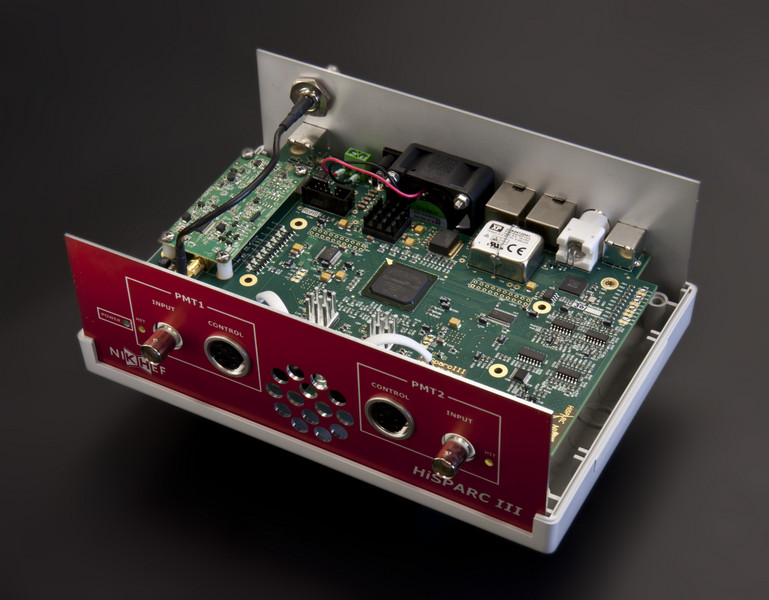
\includegraphics[scale=1.5]{Figures/8cee5cc97a}
\par\end{centering}

\caption{De HiSPARC master unit, foto uit {[}1{]}. In de blokken PMT 1 en PMT
2 zijn twee gele ledjes te zien. Deze lichten op als er straling door
respectievelijk detector 1 of detector 2 wordt gemeten. In de praktijk
worden de detectoren ongeveer iedere \SI{10}{\milli\second} geraakt.
Achter de koelgaten is een witte led te zien. Deze licht op als beide
detectoren binnen een tijdsinterval van \SI{1.5}{\micro\second} straling
waarnemen, dit komt veel minder vaak voor.}
\end{figure}



\subsection{De nauwkeurigheid van het meten van events}

Een \textit{event} vindt plaats als het station getriggerd wordt.
Bij een tweeplaatsstation wordt het station getriggerd als beide detectoren
binnen \SI{1,5}{\micro\second} een signaal lager dan \SI{-70}{\milli\volt}
afgeven. Een vierplaatsstation wordt ook getriggerd als drie detectoren
binnen \SI{1,5}{\micro\second} een signaal lager dan \SI{-30}{\milli\volt}
afgeven. Als het station getriggerd wordt, licht er een witte led
achter de koelgaten van het HiSPARC kastje op. De tijd van het event
is de tijd waarop aan de triggervoorwaarde is voldaan, dit is dus
de tweede of derde tijd van een single.

\begin{minipage}[t]{1\columnwidth}%

\paragraph{Opdracht 1:}

\textit{Bepaal 5 maal hoe vaak het witte ledje in 1 minuut oplicht
en vul dit hieronder in de tabel in.}

\begin{tabular}{|>{\centering}p{2cm}|>{\centering}p{2cm}|>{\centering}p{2cm}|>{\centering}p{2cm}|>{\centering}p{2cm}|>{\centering}p{2cm}|>{\centering}p{2cm}|}
\cline{2-7} 
\multicolumn{1}{>{\centering}p{2cm}|}{} & 1 & 2 & 3 & 4 & 5 & $N_{gem.}$\tabularnewline
\hline 
$N$ &  &  &  &  &  & \tabularnewline
\hline 
\end{tabular}%
\end{minipage}

\bigskip{}


\begin{minipage}[t]{1\columnwidth}%

\paragraph{Opdracht 2:}

\textit{Bepaal naast het gemiddelde ook de maximale en de minimale
waarde, leg uit welke nauwkeurigheid je verwacht.}

\begin{tabular}{>{\raggedright}p{16.6cm}}
\tabularnewline
\hline 
\tabularnewline
\hline 
\tabularnewline
\hline 
\tabularnewline
\hline 
\end{tabular}%
\end{minipage}

\bigskip{}


De nauwkeurigheid (spreiding) is ook wiskundig te bepalen.

\begin{minipage}[t]{1\columnwidth}%

\paragraph{Opdracht 3:}

\textit{Wiskundig is de spreiding $\sigma$ uit te rekenen, bereken
eerst het gemiddelde van $N^{2}$.}

\bigskip{}


\begin{tabular}{|>{\centering}p{2cm}|>{\centering}p{2cm}|>{\centering}p{2cm}|>{\centering}p{2cm}|>{\centering}p{2cm}|>{\centering}p{2cm}|>{\centering}p{2cm}|}
\cline{2-7} 
\multicolumn{1}{>{\centering}p{2cm}|}{} & 1 & 2 & 3 & 4 & 5 & $\left(N^{2}\right)_{gem}$\tabularnewline
\hline 
$N^{2}$ &  &  &  &  &  & \tabularnewline
\hline 
\end{tabular}

\bigskip{}


\begin{tabular}{>{\raggedright}p{16.6cm}}
\textit{De spreiding is nu te berekenen met }$\sigma=\sqrt{\left(N^{2}\right)_{gem}-\left(N_{gem}\right)^{2}}$,
\textit{dit is dus de wortel uit het gemiddelde van de kwadraten min
het kwadraat van het gemiddelde. }($N_{gem}$ \textit{is al in opdracht
1 berekend.)}\tabularnewline
\tabularnewline
\hline 
\end{tabular}%
\end{minipage}

\bigskip{}


\begin{minipage}[t]{1\columnwidth}%

\paragraph{Opdracht 4:}

\textit{Welke conclusie mag je trekken als je de waarden die je bij
opdracht 2 en 3 hebt gevonden vergelijkt?}

\begin{tabular}{>{\raggedright}p{16.6cm}}
\tabularnewline
\hline 
\tabularnewline
\hline 
\tabularnewline
\hline 
\tabularnewline
\hline 
\end{tabular}%
\end{minipage}


\subsection{Controle van de hypothese}

Het signaal van een enkele detector -een single- wordt gezien als
achtergrondstraling. De gelijktijdige signalen van twee detectoren
-een event- wijzen op een air-shower. Beide delen van de hypothese
zijn natuurlijk te onderzoeken.


\subsubsection{Het signaal van een enkele detector wordt gezien als achtergrondstraling.}

Hoe groot is de kans dat het station wordt getriggerd door achtergrondstraling?
De detector geeft alleen een signaal af als er een deeltje door de
detector gaat. Om van een air-shower te spreken moeten de deeltjes
binnen een triggervenster van \SI{1.5}{\micro\second} gedetecteerd
worden. De achtergrondstraling zorgt dat gemiddeld ongeveer iedere
10ms een deeltje door een detector van \SI{0.500}{\meter} bij \SI{1.000}{\meter}
schiet%
\footnote{Als er op school een Geigerteller is, kan de achtergrondstraling in
$\mathrm{\left[pulsen/s/m^{2}\right]}$ ook worden gemeten. Naast
het aantal pulsen per seconde is dus ook het oppervlak van de detector
van belang.%
}. Als deze singles netjes verdeeld zouden zijn, is de kans op een
tweede toevallig gemeten deeltje van de achtergrondstraling binnen
het triggervenster van \SI{1.5}{\micro\second} te berekenen.

\begin{minipage}[t]{1\columnwidth}%

\paragraph{Opdracht 5:}

\textit{Bereken (met een boxplot) hoe groot de kans is dat er een
tweede radioactief verval binnen \SI{1.5}{\micro\second} van de eerste
radioactief verval optreed:}

\begin{tabular}{>{\raggedright}p{16.6cm}}
\tabularnewline
\hline 
\tabularnewline
\hline 
\tabularnewline
\hline 
\tabularnewline
\hline 
\end{tabular}%
\end{minipage}

\bigskip{}


Een nettere manier om deze kans te berekenen is in 1838 door Siméon
Poisson {[}2{]} gepubliceerd:

\begin{equation}
P_{k}=\frac{\lambda^{k}}{k!}e^{-\lambda}
\end{equation}


Hierin is $k=1$ als een tweede detector precies éénmaal getriggerd
wordt. $\lambda$ is hier de frequentie van de achtergrondstraling
maal de duur van het triggervenster $\left(\lambda=f_{single}*T_{venster}\right)$. 

\begin{minipage}[t]{1\columnwidth}%

\paragraph{Opdracht 6:}

\textit{Laat zien dat de met de boxplot berekende waarde nauwelijks
afwijkt van de met de Poisson-formule berekende waarde $P_{k=1}$.}

\begin{tabular}{>{\raggedright}p{16.6cm}}
\tabularnewline
\hline 
\tabularnewline
\hline 
\tabularnewline
\hline 
\tabularnewline
\hline 
\end{tabular}%
\end{minipage}

\bigskip{}


Eventueel geldt bij een toevallige trigger ook $k=2$, $k=3$ etc.
In het algemeen nemen we $k>0$ (met $k\mathbb{\in N}$). De kans
dat er GEEN toevallige trigger optreedt is $P_{k=0}$.

\begin{minipage}[t]{1\columnwidth}%

\paragraph{Opdracht 7:}

\textit{Met de kans dat er geen toevallige trigger optreed, is de
kans op een toevallige trigger ook te berekenen. (De kans op een trigger
plus de kans op geen trigger is 100\%.) Bereken deze kans:}

\begin{tabular}{>{\raggedright}p{16.6cm}}
\tabularnewline
\hline 
\tabularnewline
\hline 
\tabularnewline
\hline 
\tabularnewline
\hline 
\end{tabular}%
\end{minipage}

\bigskip{}


De duur van het triggervenster is van belang als we naar de kans op
toevallige triggers kijken. We kunnen een grafiek maken van de kans
op een toevallige trigger als functie van de duur van het triggervenster
$T_{venster}$. Er geldt: $\lambda=f_{single}*T_{venster}$, en dit
geval wordt dit: $\lambda=100*T_{venster}$$ $. 

\begin{minipage}[t]{1\columnwidth}%

\paragraph{Opdracht 8:}

\textit{Maak de onderstaande tabel voor een station met twee detectoren
af:}

\bigskip{}


\begin{tabular}{|c|>{\centering}p{1cm}|>{\centering}p{1cm}|>{\centering}p{1cm}|>{\centering}p{1cm}|>{\centering}p{1cm}|>{\centering}p{1cm}|>{\centering}p{1cm}|}
\hline 
$T_{venster}$ {[}$\mu\mathrm{s}${]} & 1,5 & 3,0 & 7,5 & 15 & 30 & 75 & 150\tabularnewline
\hline 
$P_{trigger}=1-P_{k=0}$ &  &  &  &  &  &  & \tabularnewline
\hline 
\end{tabular}%
\end{minipage}

\bigskip{}


\begin{figure}[h]

\paragraph{Opdracht 9:}

\textit{Maak het diagram van de kans op een toevallige trigger als
functie van de duur van het triggervenster.\bigskip{}
}

\begin{tabular}{|>{\centering}p{0.1cm}|>{\centering}p{0.1cm}|>{\centering}p{0.1cm}|>{\centering}p{0.1cm}|>{\centering}p{0.1cm}|>{\centering}p{0.1cm}|>{\centering}p{0.1cm}|>{\centering}p{0.1cm}|>{\centering}p{0.1cm}|>{\centering}p{0.1cm}|>{\centering}p{0.1cm}|>{\centering}p{0.1cm}|>{\centering}p{0.1cm}|>{\centering}p{0.1cm}|>{\centering}p{0.1cm}|>{\centering}p{0.1cm}|>{\centering}p{0.1cm}|>{\centering}p{0.1cm}|>{\centering}p{0.1cm}|>{\centering}p{0.1cm}|>{\centering}p{0.1cm}|>{\centering}p{0.1cm}|>{\centering}p{0.1cm}|>{\centering}p{0.1cm}|>{\centering}p{0.1cm}|>{\centering}p{0.1cm}|>{\centering}p{0.1cm}|>{\centering}p{0.1cm}|>{\centering}p{0.1cm}|}
\hline 
 &  &  &  &  &  &  &  &  &  &  &  &  &  &  &  &  &  &  &  &  &  &  &  &  &  &  &  & \tabularnewline
\hline 
 &  &  &  &  &  &  &  &  &  &  &  &  &  &  &  &  &  &  &  &  &  &  &  &  &  &  &  & \tabularnewline
\hline 
 &  &  &  &  &  &  &  &  &  &  &  &  &  &  &  &  &  &  &  &  &  &  &  &  &  &  &  & \tabularnewline
\hline 
 &  &  &  &  &  &  &  &  &  &  &  &  &  &  &  &  &  &  &  &  &  &  &  &  &  &  &  & \tabularnewline
\hline 
 &  &  &  &  &  &  &  &  &  &  &  &  &  &  &  &  &  &  &  &  &  &  &  &  &  &  &  & \tabularnewline
\hline 
 &  &  &  &  &  &  &  &  &  &  &  &  &  &  &  &  &  &  &  &  &  &  &  &  &  &  &  & \tabularnewline
\hline 
 &  &  &  &  &  &  &  &  &  &  &  &  &  &  &  &  &  &  &  &  &  &  &  &  &  &  &  & \tabularnewline
\hline 
 &  &  &  &  &  &  &  &  &  &  &  &  &  &  &  &  &  &  &  &  &  &  &  &  &  &  &  & \tabularnewline
\hline 
 &  &  &  &  &  &  &  &  &  &  &  &  &  &  &  &  &  &  &  &  &  &  &  &  &  &  &  & \tabularnewline
\hline 
 &  &  &  &  &  &  &  &  &  &  &  &  &  &  &  &  &  &  &  &  &  &  &  &  &  &  &  & \tabularnewline
\hline 
 &  &  &  &  &  &  &  &  &  &  &  &  &  &  &  &  &  &  &  &  &  &  &  &  &  &  &  & \tabularnewline
\hline 
 &  &  &  &  &  &  &  &  &  &  &  &  &  &  &  &  &  &  &  &  &  &  &  &  &  &  &  & \tabularnewline
\hline 
 &  &  &  &  &  &  &  &  &  &  &  &  &  &  &  &  &  &  &  &  &  &  &  &  &  &  &  & \tabularnewline
\hline 
 &  &  &  &  &  &  &  &  &  &  &  &  &  &  &  &  &  &  &  &  &  &  &  &  &  &  &  & \tabularnewline
\hline 
 &  &  &  &  &  &  &  &  &  &  &  &  &  &  &  &  &  &  &  &  &  &  &  &  &  &  &  & \tabularnewline
\hline 
 &  &  &  &  &  &  &  &  &  &  &  &  &  &  &  &  &  &  &  &  &  &  &  &  &  &  &  & \tabularnewline
\hline 
 &  &  &  &  &  &  &  &  &  &  &  &  &  &  &  &  &  &  &  &  &  &  &  &  &  &  &  & \tabularnewline
\hline 
 &  &  &  &  &  &  &  &  &  &  &  &  &  &  &  &  &  &  &  &  &  &  &  &  &  &  &  & \tabularnewline
\hline 
\end{tabular}
\end{figure}


\bigskip{}


Tot nu toe zijn we uitgegaan van een station met twee detectoren.
Bij een station met vier detectoren zijn er logischerwijs twee detectoren
meer.

\begin{minipage}[t]{1\columnwidth}%

\paragraph{Opdracht 10:}

\textit{Beredeneer hoe groot de kans op een toevallige trigger is
bij een station met 4 detectoren en een triggervenster van \SI{1.5}{\micro\second}
(Denk aan het aantal mogelijke combinaties!):}

\begin{tabular}{>{\raggedright}p{16.6cm}}
\tabularnewline
\hline 
\tabularnewline
\hline 
\tabularnewline
\hline 
\tabularnewline
\hline 
\end{tabular}%
\end{minipage}

\bigskip{}



\subsubsection{De gelijktijdige signalen van twee detectoren wijzen op een air-shower.}

Een experimenteel onderzoek leidt hier het snelst tot inzicht. In
figuur \ref{fig:Meetstations} is een plattegrond te zien. Hierop
zijn zowel een station met 2 detectoren als een station met 4 detectoren
te zien. De plattegrond past in de deksel van een papierdoos. Op de
plattegrond zijn de scintillatorplaten van \SI{0.500}{\meter} bij
\SI{1.000}{\meter} op schaal getekend. 

\noindent \begin{center}
\begin{figure}[p]
\noindent \begin{centering}
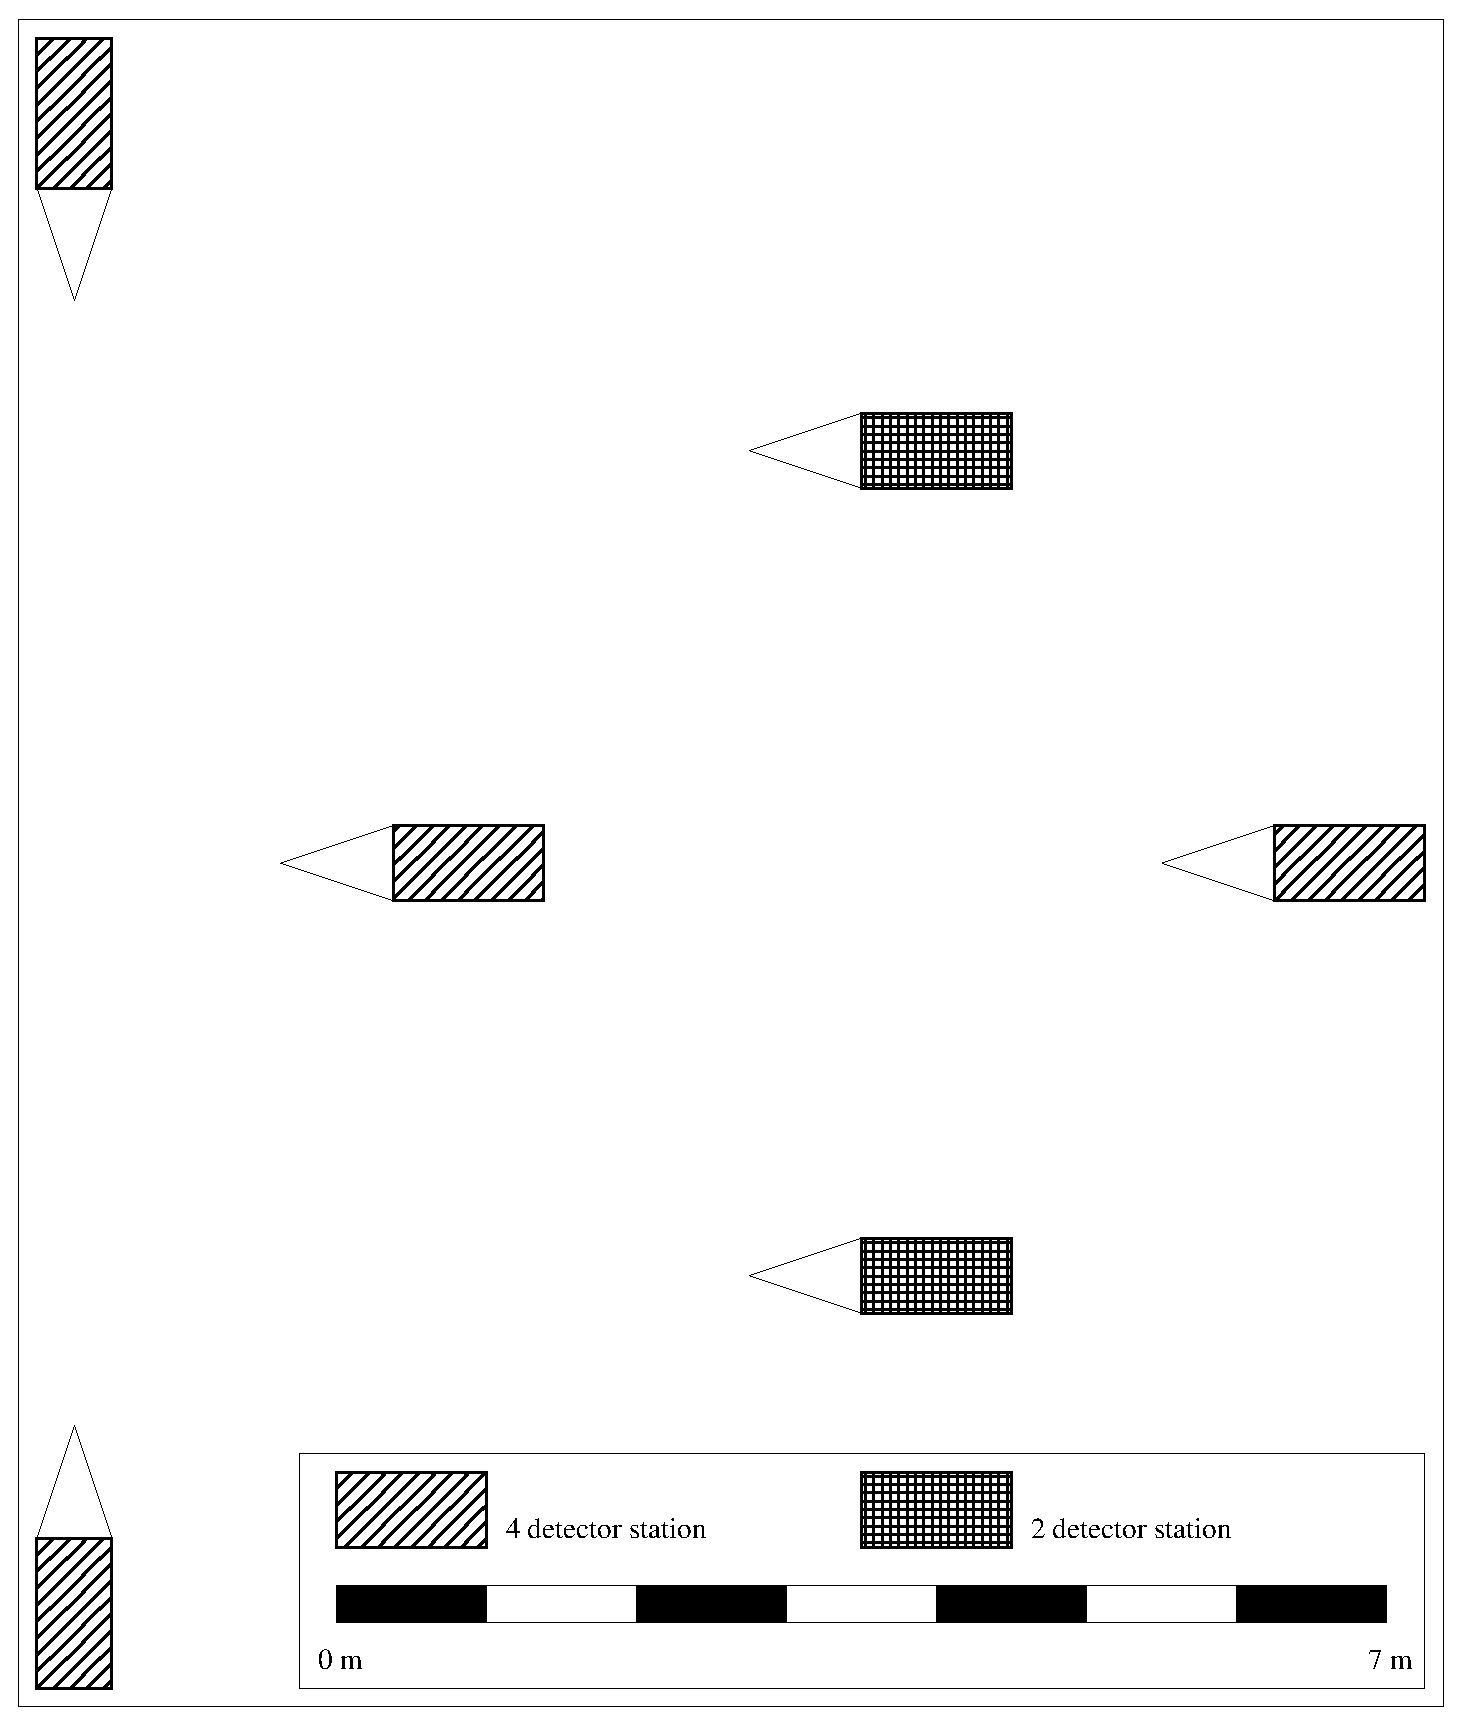
\includegraphics[width=15.833cm]{Figures/station}
\par\end{centering}

\caption{\label{fig:Meetstations}Een meetstation met twee detectoren en een
meetstation met vier detectoren.}
\end{figure}

\par\end{center}

\begin{minipage}[t]{1\columnwidth}%

\paragraph{Opdracht 11:}

\textit{Bepaal het oppervlak in de doos in $\mathrm{cm^{2}}$. In
werkelijkheid komt dit overeen met een oppervlak in $\mathrm{m^{2}}$,
dit tweede oppervlak is te berekenen.}

\begin{tabular}{>{\raggedright}p{16.6cm}}
\tabularnewline
\hline 
\tabularnewline
\hline 
\tabularnewline
\hline 
\tabularnewline
\hline 
\end{tabular}%
\end{minipage}\bigskip{}
We willen de kans bepalen dat een air-shower gedetecteerd wordt. Deze
hangt kans hangt af van de deeltjesdichtheid $\rho$, het aantal deeltjes
per $\mathrm{m^{2}}$ in de air-shower. Deze deeltjes simuleren we
met korreltjes couscous.

\begin{minipage}[t]{1\columnwidth}%

\paragraph{Opdracht 12:}

\textit{Bereken hoeveel deeltjes nodig zijn:}

\bigskip{}


\begin{tabular}{|>{\centering}p{3cm}|>{\centering}p{2cm}|>{\centering}p{2cm}|>{\centering}p{2cm}|>{\centering}p{2cm}|>{\centering}p{2cm}|}
\hline 
$\rho_{werkelijk}$ $\left[\mathrm{m^{-2}}\right]$ & 0,5 & 1 & 2 & 5 & 10\tabularnewline
\hline 
Aantal korreltjes in de doos &  &  &  &  & \tabularnewline
\hline 
\end{tabular}%
\end{minipage}

\bigskip{}
Het wordt een heel karwei om de korreltjes te tellen. We wegen een
aantal korreltjes en bereken de massa couscous die nodig is.

\begin{minipage}[t]{1\columnwidth}%

\paragraph{Opdracht 13:}

\textit{Bereken de massa couscous:}

\bigskip{}


\begin{tabular}{|>{\centering}p{3cm}|>{\centering}p{2cm}|>{\centering}p{2cm}|>{\centering}p{2cm}|>{\centering}p{2cm}|>{\centering}p{2cm}|}
\hline 
$\rho_{werkelijk}$ $\left[\mathrm{m^{-2}}\right]$ & 0,5 & 1 & 2 & 5 & 10\tabularnewline
\hline 
Massa couscous in de doos &  &  &  &  & \tabularnewline
\hline 
\end{tabular}%
\end{minipage}

\bigskip{}


Nu kunnen we de hoeveelheid couscous in de doos doen die overeenkomt
met 0,5 deeltjes per $\mathrm{m^{2}}$ in werkelijkheid. We schudden
de doos en proberen de couscous zo gelijkmatig te verdelen. Als er
op twee detectoren van een station minstens 1 korreltje ligt is het
station getriggerd. Let op dat je niet iedere keer schudt tot er ,,toevallig''
een trigger wordt afgegeven. Dit is een aantal malen te herhalen en
we kunnen aanvinken of het ,,station'' getriggerd wordt of niet.
Let op, één detector kan per keer maximaal een tiental deeltjes meten,
daarna meet het station niets extra's meer.

\begin{minipage}[t]{1\columnwidth}%

\paragraph{Opdracht 14:}

\textit{Voer het experiment een aantal malen uit en bepaal de kans
dat het station getriggerd wordt.}

\bigskip{}


\begin{tabular}{|>{\centering}p{2.2cm}|>{\centering}p{1cm}|>{\centering}p{1cm}|>{\centering}p{1cm}|>{\centering}p{1cm}|>{\centering}p{1cm}|>{\centering}p{1cm}|>{\centering}p{1cm}|>{\centering}p{1cm}|>{\centering}p{1cm}|>{\centering}p{1cm}|}
\cline{2-11} 
\multicolumn{1}{>{\centering}p{2.2cm}|}{} & \multicolumn{5}{c|}{twee detectoren} & \multicolumn{5}{c|}{vier detectoren}\tabularnewline
\hline 
$\rho$ $\left[\mathrm{m^{-2}}\right]$ & 0,5 & 1 & 2 & 5 & 10 & 0,5 & 1 & 2 & 5 & 10\tabularnewline
\hline 
meting 1 &  &  &  &  &  &  &  &  &  & \tabularnewline
\hline 
meting 2 &  &  &  &  &  &  &  &  &  & \tabularnewline
\hline 
meting 3 &  &  &  &  &  &  &  &  &  & \tabularnewline
\hline 
meting 4 &  &  &  &  &  &  &  &  &  & \tabularnewline
\hline 
meting 5 &  &  &  &  &  &  &  &  &  & \tabularnewline
\hline 
meting 6 &  &  &  &  &  &  &  &  &  & \tabularnewline
\hline 
meting 7 &  &  &  &  &  &  &  &  &  & \tabularnewline
\hline 
meting 8 &  &  &  &  &  &  &  &  &  & \tabularnewline
\hline 
meting 9 &  &  &  &  &  &  &  &  &  & \tabularnewline
\hline 
meting 10 &  &  &  &  &  &  &  &  &  & \tabularnewline
\hline 
triggerkans &  &  &  &  &  &  &  &  &  & \tabularnewline
\hline 
\end{tabular}%
\end{minipage}

\bigskip{}


Met deze gegevens is een diagram voor de triggerkans als functie van
de deeltjesdichtheid te maken.

\begin{figure}[h]

\paragraph{Opdracht 15:}

\textit{Maak het diagram voor een station met twee en een station
met vier detectoren.\bigskip{}
}

\begin{tabular}{|>{\centering}p{0.1cm}|>{\centering}p{0.1cm}|>{\centering}p{0.1cm}|>{\centering}p{0.1cm}|>{\centering}p{0.1cm}|>{\centering}p{0.1cm}|>{\centering}p{0.1cm}|>{\centering}p{0.1cm}|>{\centering}p{0.1cm}|>{\centering}p{0.1cm}|>{\centering}p{0.1cm}|>{\centering}p{0.1cm}|>{\centering}p{0.1cm}|>{\centering}p{0.1cm}|>{\centering}p{0.1cm}|>{\centering}p{0.1cm}|>{\centering}p{0.1cm}|>{\centering}p{0.1cm}|>{\centering}p{0.1cm}|>{\centering}p{0.1cm}|>{\centering}p{0.1cm}|>{\centering}p{0.1cm}|>{\centering}p{0.1cm}|>{\centering}p{0.1cm}|>{\centering}p{0.1cm}|>{\centering}p{0.1cm}|>{\centering}p{0.1cm}|>{\centering}p{0.1cm}|>{\centering}p{0.1cm}|}
\hline 
 &  &  &  &  &  &  &  &  &  &  &  &  &  &  &  &  &  &  &  &  &  &  &  &  &  &  &  & \tabularnewline
\hline 
 &  &  &  &  &  &  &  &  &  &  &  &  &  &  &  &  &  &  &  &  &  &  &  &  &  &  &  & \tabularnewline
\hline 
 &  &  &  &  &  &  &  &  &  &  &  &  &  &  &  &  &  &  &  &  &  &  &  &  &  &  &  & \tabularnewline
\hline 
 &  &  &  &  &  &  &  &  &  &  &  &  &  &  &  &  &  &  &  &  &  &  &  &  &  &  &  & \tabularnewline
\hline 
 &  &  &  &  &  &  &  &  &  &  &  &  &  &  &  &  &  &  &  &  &  &  &  &  &  &  &  & \tabularnewline
\hline 
 &  &  &  &  &  &  &  &  &  &  &  &  &  &  &  &  &  &  &  &  &  &  &  &  &  &  &  & \tabularnewline
\hline 
 &  &  &  &  &  &  &  &  &  &  &  &  &  &  &  &  &  &  &  &  &  &  &  &  &  &  &  & \tabularnewline
\hline 
 &  &  &  &  &  &  &  &  &  &  &  &  &  &  &  &  &  &  &  &  &  &  &  &  &  &  &  & \tabularnewline
\hline 
 &  &  &  &  &  &  &  &  &  &  &  &  &  &  &  &  &  &  &  &  &  &  &  &  &  &  &  & \tabularnewline
\hline 
 &  &  &  &  &  &  &  &  &  &  &  &  &  &  &  &  &  &  &  &  &  &  &  &  &  &  &  & \tabularnewline
\hline 
 &  &  &  &  &  &  &  &  &  &  &  &  &  &  &  &  &  &  &  &  &  &  &  &  &  &  &  & \tabularnewline
\hline 
 &  &  &  &  &  &  &  &  &  &  &  &  &  &  &  &  &  &  &  &  &  &  &  &  &  &  &  & \tabularnewline
\hline 
 &  &  &  &  &  &  &  &  &  &  &  &  &  &  &  &  &  &  &  &  &  &  &  &  &  &  &  & \tabularnewline
\hline 
 &  &  &  &  &  &  &  &  &  &  &  &  &  &  &  &  &  &  &  &  &  &  &  &  &  &  &  & \tabularnewline
\hline 
 &  &  &  &  &  &  &  &  &  &  &  &  &  &  &  &  &  &  &  &  &  &  &  &  &  &  &  & \tabularnewline
\hline 
 &  &  &  &  &  &  &  &  &  &  &  &  &  &  &  &  &  &  &  &  &  &  &  &  &  &  &  & \tabularnewline
\hline 
 &  &  &  &  &  &  &  &  &  &  &  &  &  &  &  &  &  &  &  &  &  &  &  &  &  &  &  & \tabularnewline
\hline 
 &  &  &  &  &  &  &  &  &  &  &  &  &  &  &  &  &  &  &  &  &  &  &  &  &  &  &  & \tabularnewline
\hline 
 &  &  &  &  &  &  &  &  &  &  &  &  &  &  &  &  &  &  &  &  &  &  &  &  &  &  &  & \tabularnewline
\hline 
 &  &  &  &  &  &  &  &  &  &  &  &  &  &  &  &  &  &  &  &  &  &  &  &  &  &  &  & \tabularnewline
\hline 
\end{tabular}

\bigskip{}


\caption{Het diagram van de triggerkans als functie van $\rho$}
\end{figure}



\section{Coïncidenties}

Een event vindt plaats als twee of meerdere detectoren van een station
nagenoeg tegelijkertijd worden getriggerd. Dit gebeurt al met relatief
kleine air-showers. Een grotere air-shower%
\footnote{De grote van de voetafdruk van de air-shower op Aarde is een maat
voor de hoeveelheid energie van het primaire kosmische deeltje dat
als eerste de atmosfeer raakt.%
} kan deeltjes over een groter oppervlak verspreiden. In dit grotere
oppervlak kunnen meerdere stations liggen. Als meerdere stations nagenoeg
tegelijk worden getriggerd, spreken we van een coïncidentie. 

Als een coïncidentie door een enkele air-shower wordt veroorzaakt,
moeten de metingen aan een aantal randvoorwaarden voldoen. Deeltjes
kunnen niet sneller dan de lichtsnelheid bewegen. De locaties van
de stations zijn bekend. Als een station getriggerd wordt, wordt deze
tijd binnen het station op \SI{2.5}{\nano\second} nauwkeurig opgeslagen.
Tussen stations onderling geldt een nauwkeurigheid van \SI{15}{\nano\second}.
Omdat de afstand tussen de stations bekend is, is er een vrij klein
tijdvenster waarbinnen de detectoren deeltjes kunnen meten. Met de
afstanden tussen de stations en de triggertijden is het zelfs mogelijk
om de richting van de air-shower te bepalen {[}3{]}.

\bigskip{}


\begin{minipage}[t]{1\columnwidth}%

\paragraph{Opdracht 16}

\textit{Ook bij coïncidenties kan een triggervenster worden gebruikt.
Dit venster hangt af van de afstand tussen de stations en de lichtsnelheid.
De air-shower geeft het grootste tijdverschil als deze horizontaal
door de opstelling beweegt. Een dergelijke air-shower wordt gegenereerd
door een primair kosmisch deeltje met een extreem grote energie. In
de praktijk komen deze air-showers zelden voor. }

\textit{Bereken de grootte van het triggervenster in de volgende gevallen:}

\bigskip{}


\begin{tabular}{|c|>{\centering}p{1.5cm}|>{\centering}p{1.5cm}|>{\centering}p{1.5cm}|>{\centering}p{1.5cm}|}
\hline 
Afstand tussen de stations {[}m{]} & 100 & 200 & 500 & 1000\tabularnewline
\hline 
Duur van het triggervenster {[}ns{]} &  &  &  & \tabularnewline
\hline 
\end{tabular}%
\end{minipage}

\newpage{}


\subsection{Tijdsverschillen tussen stations}

De gemeten tijd van de verschillende stations heeft een nauwkeurigheid
van \SI{15}{\nano\second}. Als we uitgaan van de hypothese dat de
kosmische straling in dezelfde mate vanuit ieder punt aan de hemel
komt en de klokken allemaal goed lopen, zal het gemiddelde tijdsverschil
bij een voldoende grote steekproef \SI{0}{\nano\second} moeten zijn.
Als er een tijdsverschil gemeten wordt, lopen de klokken niet synchroon.
We kunnen zelfs bepalen hoeveel de klokken voor of achter lopen. Dit
kan door gebruik te maken van event gegevens van een aantal stations. 

Deze zijn bijvoorbeeld op te vragen met:

\texttt{\small{http://data.hisparc.nl/data/501/events?start=2013-08-01+00:00:00\&end=2013-08-01+01:00:00}}. 

Het stationnummer (501), het startmoment (datum (2013-08-01) en tijd
(00:00:00)) en het stopmoment (datum (2013-08-01) en tijd (01:00:00))
worden in de url%
\footnote{Unified Resource Locator: het internet adres.%
} meegestuurd, hier zijn ook andere stationnummers, data en tijden
in te vullen%
\footnote{In principe kan een grote periode worden opgevraagd. Begin echter
met een uur, het opvragen van een dag voor meerdere stations duurt
wel even.%
}. De server stuurt een csv%
\footnote{Comma Seperated Value: de waarden kunnen door komma's gescheiden zijn,
dit is niet altijd het geval. In dit bestand worden ,,tabs'' gebruikt.%
}-bestand met event gegevens terug. Dit bestand is in een spreadsheet
maar ook in een javascript programma te openen. 

Om de verschiltijden te bepalen kan de volgende procedure gevolgd
worden:
\begin{itemize}
\item Geef de stations namen, bijvoorbeeld a, b, c, etc.
\item Neem de eerste tijd van station a en kijk of er binnen het venster
events van de stations b, c, etc. zijn. Schrijf de verschiltijden
van a met b, c, etc. op en verwijder de eerste tijd uit de lijst van
station a.
\item Neem de eerste tijd van station b en kijk of er binnen het venster
events van de stations c, etc. zijn. Schrijf de verschiltijden van
b met c, etc. op en verwijder de eerste tijd uit de lijst van station
b.
\item Herhaal dit tot het een na laatste station.
\item Begin overnieuw bij station a met de kortere lijst en herhaal alles
tot de lijsten leeg zijn.
\item We hebben nu verschillijsten van a en b, a en c, etc. Er zijn ook
verschillijsten van b en c, etc. Met deze lijsten zijn histogrammen
te maken. 
\end{itemize}
We weten dat stations niet nauwkeuriger kunnen meten dan \SI{2,5}{\nano\second}.
Karl Pearson (1857-1936) {[}4{]} ontwikkelde een methode om met lijsten
gebeurtenissen een histogram te maken. In dit geval gaan we uit van
het aantal verschiltijden (de frequentie van verschiltijden) tussen
twee grenzen (de bin-waarden). Een reeks grenzen levert een reeks
frequenties op. Hiermee is een histogram of staafdiagram te maken.
We kunnen de grenzen bijvoorbeeld zo vastleggen:

\bigskip{}
\begin{tabular}{|c|c|c|c|c|c|c|c|c|}
\hline 
Bin-waarde {[}ns{]} & eerder & -7,5 tot 5 & -5 tot -2,5 & -2,5 tot 0 & 0 tot 2,5 & 2,5 tot 5 & 5 tot 7,5 & later\tabularnewline
\hline 
Frequentie &  &  &  &  &  &  &  & \tabularnewline
\hline 
\end{tabular}

\bigskip{}


Het maken van een dergelijke tabel is een behoorlijke klus met een
spreadsheet programma. Het uiteindelijke histogram is langs de horizontale
as te verdelen in bin-waarden. Langs de verticale as komen de frequenties
te staan. In het ideale geval ligt het maximum bij \SI{0}{\nano\second}.
In de praktijk zal dit zelden het geval zijn.

\bigskip{}


\begin{minipage}[t]{1\columnwidth}%

\paragraph{Opdracht 17}

\textit{Het bepalen van de bin-breedte -de afstand tussen de bin-waarden-
verdient enige aandacht. Als de frequentie van verschilwaarden laag
is, is het niet handig om een kleine bin-breedte te nemen. De frequentie
hangt namelijk af van de bin-breedte. Een kleine bin-breedte geeft
een lage frequentie, maar een grote nauwkeurigheid in de tijd. Een
grote bin-breedte geeft een hoge frequentie maar een kleine nauwkeurigheid
in de tijd.}

\textit{Bedenk een methode om de bin-breedte handig te kiezen als
het totale aantal verschiltijden (coïncidenties) (N) en de minimale
($t_{min}$) en maximale ($t_{max}$) bin-waarde bekend zijn:}

\begin{tabular}{>{\raggedright}p{16.6cm}}
\tabularnewline
\hline 
\tabularnewline
\hline 
\tabularnewline
\hline 
\tabularnewline
\hline 
\end{tabular}%
\end{minipage}


\section*{Referenties}

{[}1{]} https://www.nikhef.nl/wetenschap-techniek/technische-afdelingen/elektronicatechnologie/projecten/

{[}2{]}, {[}4{]} wikipedia

{[}3{]} Richting Reconstructie, C.G.N. van Veen
\end{document}
